% **************************************************
%   Wichtig für die verwendung der hsrmreport-Klasse!
%   
%   Die Datei hsrmreport.cls muss in dem selben Ordner sein
%   wie die .tex Datei die diese Klasse verwenden möchte.
%
%   Desweiteren ist die Dokumentenklasse nach aktuellem 
%   noch  Optionen, sprich Zweiseitig, änderung 
%   der Schriftgröße oder ähnliches. Ich werde versuchen 
%   diese Features hinzu zufügen sobald es mir möglich ist. 
%
%   Falls Ihr Probleme, Anregungen oder Verbesserungen habt,
%   könnt ihr mir das gerne mitteilen.
%
%   Es kann sein das ihr evtl. manche Pakete noch installieren 
%   müsst bevor die Klasse Fehlerfrei funktioniert.
%   Meldungen wie "Command terminated with space." können ignoriert werden.
%
%   Ich werde auch eine Übersicht aller Pakete schreiben, die ich verwendet habe.
%      
%
%   E-Mail: timjonas.wechler@student.hs-rm.de
% **************************************************


\documentclass{hsrmreport}
% **************************************************
% Ihr könnte die Angaben der TITELSEITE hier ändern
% **************************************************
\newcommand{\titel}{Versuch 3}
\newcommand{\studiengang}{Angewandte Pyhsik}
\newcommand{\studienrichtung}{}
\newcommand{\dokumentenart}{Praktikumsbericht}
\newcommand{\kurs}{LV:\ Elektronik 1 Praktikum}
\newcommand{\versuchsdurchfuehrung}{11. Januar 2021}

%Falls ihr weniger als vier Studenten seit könnt ihr dies Einträge die zu viel sind einfach löschen. 
%Ein Feature für das angeben der Mat.Nr. ist noch in Arbeit. 
\newcommand{\studentA}{Cassel, Niclas}
\newcommand{\matStudentA}{(1110348)}
\newcommand{\studentB}{Wechler, Tim-Jonas}
\newcommand{\matStudentB}{(1137877)}
\newcommand{\studentC}{}
\newcommand{\matStudentC}{}
\newcommand{\studentD}{}
\newcommand{\matStudentD}{}


% Mit dem Befehl \today wird immer das aktuelle Datum auf der Titelseite ausgebeben.
% Wenn dies nicht erwünscht ist einfach manuell das gewünschte Datum eintragen.
\newcommand{\datum}{\today}



\begin{document}
    % **************************************************
    %
    %   ALLES zwischen hier und dem Begin des Berichts 
    %   nicht ändern, außer ihr wisst was ihr tut ;). 
    %
    % **************************************************

    % Title 
    \frontpage%

    %Römischen Seitenzahl
    \pagenumbering{Roman}
    
    %Inhaltsverzeichnis
    \tableofcontents

    %Abbildungsverzeichnis
    \listoffigures

    %Tabellenverzeichnis
    %\listoftables

    
    \clearpage

    %Normale Seitenzahlen
    \pagenumbering{arabic}

    %Das seitenLayout mit Kapitel und Unterkapitel im Header jeder Seite des Berichts
    \pagestyle{scrheadings}

    % **************************************************
    %
    % HIER BEGINNT DER BERICHT
    %
    % **************************************************

    \chapter{Vorbereitung}
    \section{Aufbau eines Oszilloskop-Tastkopfes}
        Der Tastkopf dient als Verbindung zwischen dem Oszilloskop und der zu messenden Spannung. Es ist auch möglich ein Kabel zu verwenden, jedoch sind dann Widerstand und Kapazität bei der Messung undefiniert. Bei hohen Frequenzen wird dadurch das Messsignal verfälscht. Der Tastkopf kann die Spannung unter bekannten Bedingungen Messen.~\cite{tastkopf_deniz}
        Die Signalverarbeitung eines Tastkopfes kann mit passiven Bauelementen erfolgen oder durch eine aktive Schaltung. Wichtig ist das der Eingangswiderstand eines Tastkopfes möglichst groß und die Einkangskapazität möglichst klein ist, damit das Signal unverfälscht weitergegeben wird. Dabei gibt es viele verschiedene Tastköpfe mit eigenen Eigenschaften. Im Folgenden sind diese mit ihrem Aufbau aufgelistet.~\cite{tastkopf_wiki}

        \begin{enumerate}

        \item Standard-Tastkopf
            \begin{figure}[h!]
                \centering
                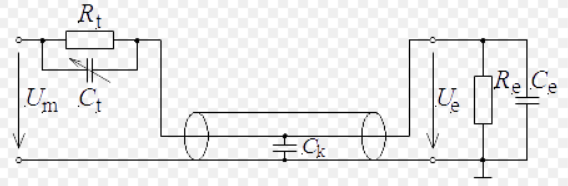
\includegraphics[]{111.PNG}
                \caption{Aufbau eines Standart Tastkopfes~\cite{tastkopf_standard}}
            \end{figure}

        \item Transmissions-Line-Tastkopf
            \begin{figure}[h!]
                \centering
                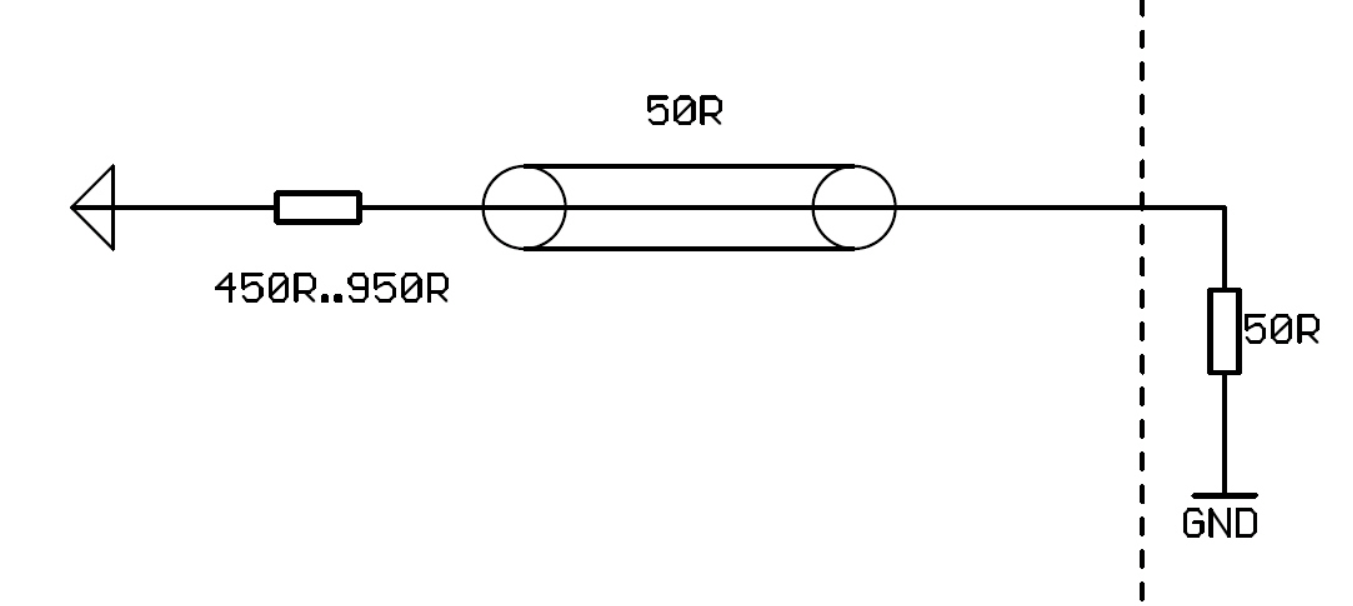
\includegraphics[width=0.5\linewidth]{112.PNG}
                \caption{Aufbau eines Transmission-Line-Tastkopfes~\cite{transmission_line_probe}}
            \end{figure}
        \newpage
        \item Aktiver Tastkopf
            \begin{figure}[h!]
                \centering
                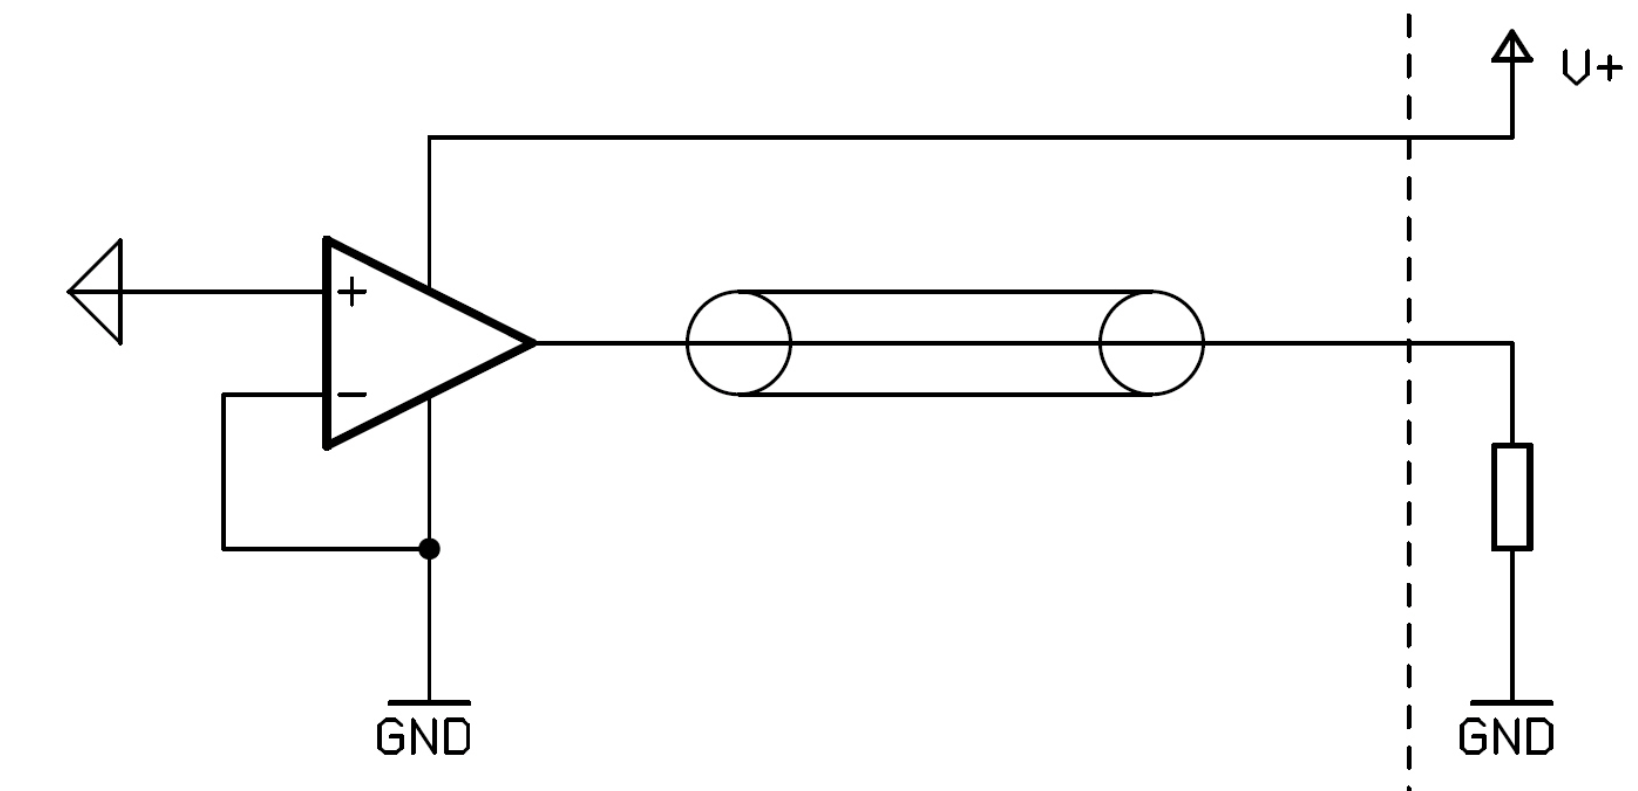
\includegraphics[width=0.5\linewidth]{113.PNG}
                \caption{Aufbau eines aktiven Tastkopfes~\cite{active_probe}}
            \end{figure}

        \item Differentieller Tastkopf
            \begin{figure}[h!]
                \centering
                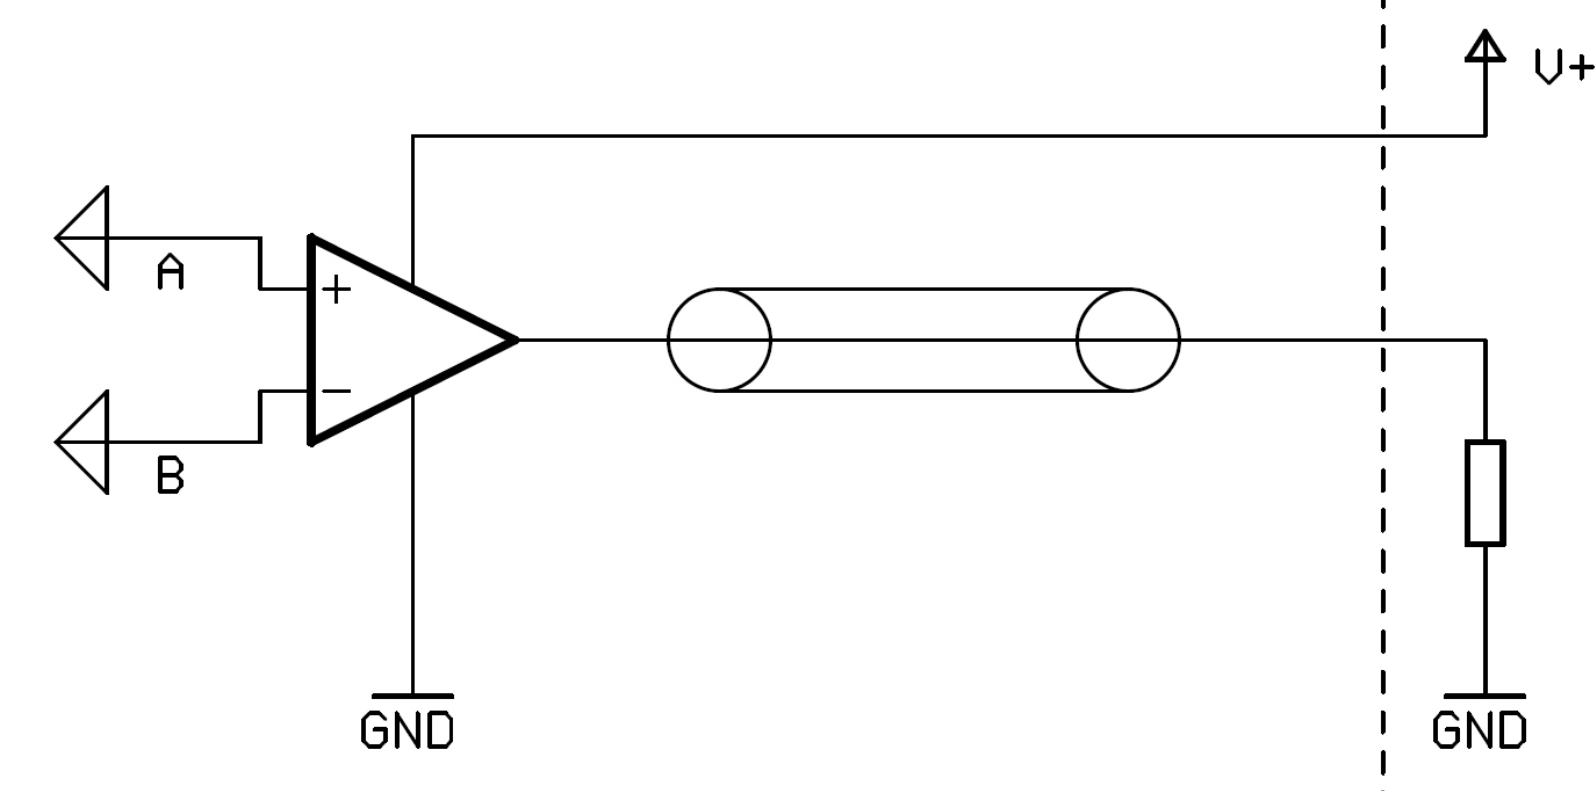
\includegraphics[width=0.5\linewidth]{114.PNG}
                \caption{Aufbau eines differentiellen Tastkopfes~\cite{differential_probe}}
            \end{figure}

        \end{enumerate}

        \begin{table}[h!]
            \centering
            \caption{Begriffserklärung für die einzelnen Buchstaben in den Abbildungen}
            \begin{tabular}{|c|c|}
                \hline
                $R_t$ & Tastkopfwiderstand\\ \hline \hline
                $C_t$ & Tastkopfkapazität \\ \hline
                $U_m$ & Spannungsmessung\\ \hline
                $C_K$ & Kabelkapazität\\ \hline
                $U_e$ & Eingangsspannung\\ \hline
                $R_e$ & Eingangswiderstand\\ \hline
                $C_e$ & Eingangskapazität\\ \hline
                Zahl mit R & Widerstand mit Zahlenwert \\ \hline
                GND & Ground (zu Erde)\\ \hline
                V & Spannung\\ \hline
            \end{tabular}
        \end{table}


    \chapter{Versuchsdurchführung}
    \section{Aufnahme der Eingangskennlinie}
        Für die Aufnahme der Eingangskennlinie  eines Transistors wird folgende Schaltung benötigt \fref{fig:21}. 
        Dabei wurde die Schaltung aus dem Versuchsaufbau etwas vereinfacht.

        \begin{figure}[!ht]
            \centering
            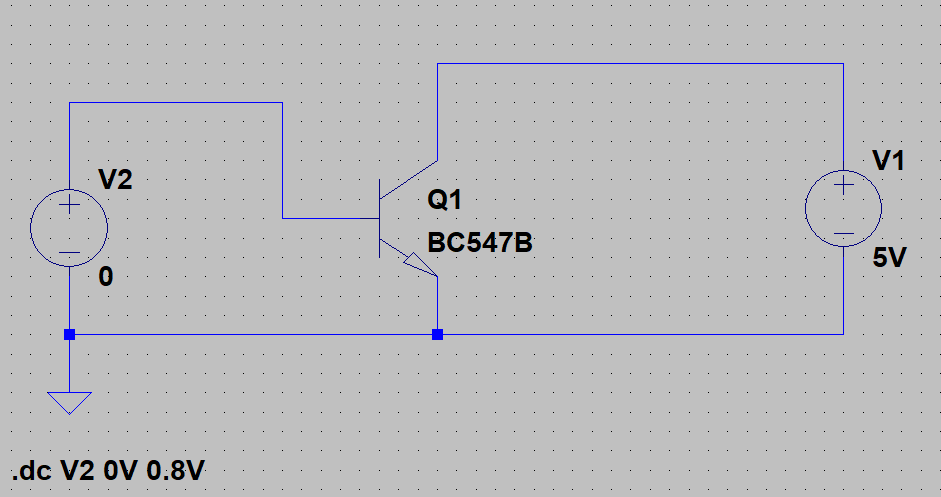
\includegraphics[width=0.5\linewidth]{Bilder/21aufbau.PNG}
            \caption{Schaltung zur Aufnahme der Eingangskennlinie}
            \label{fig:21}
        \end{figure}

        Für V1 (\(U_{CE}\)) werden 5V verwendet und V2 (\(U_{BE}\)) wird im Intervall zwischen 0 V und 0,8 V verwendet. Bei der Messung des Basisstrom \(I_B\) kamen folgende Werte heraus, welche im folgenden Graph dargestellt werden.

        \begin{figure}[!ht]
            \centering
                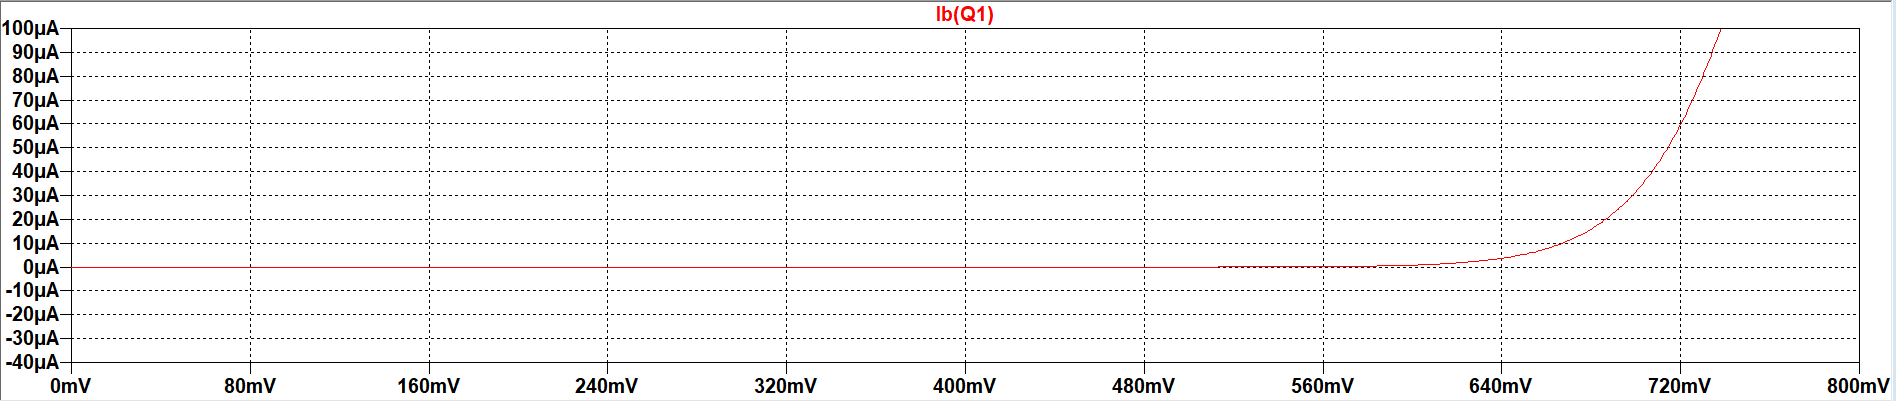
\includegraphics[width=\linewidth]{Bilder/21graph.PNG}
            \caption{Messwerte des Eingangssignals eines NPN-Transistors (Typ BC547B)}
        \end{figure}

        Der Basisstrom eines NPN-Transistors liegt bei 0 A bis bis er circa bei einer Spannung von 640 mV stark ansteigt.

        \newpage
    \section{Bestimmung des differentiellen Eingangswiderstands}
        Zur Bestimmung des differentiellen Eingangswiderstandes (\(r_{BE}\)) wird die Schaltung aus 2.1 leicht verändert. Die Spannungsquelle V2 wird durch eine Stromquelle I1 ersetzt. Die Spannungsquelle V1 bleibt bei 5 V und I1 (\(I_B\)) wird im Intervall von \(10\,nA\) bis \(100\,\mu A\) eingesetzt. 

        \begin{figure}[!ht]
            \centering
            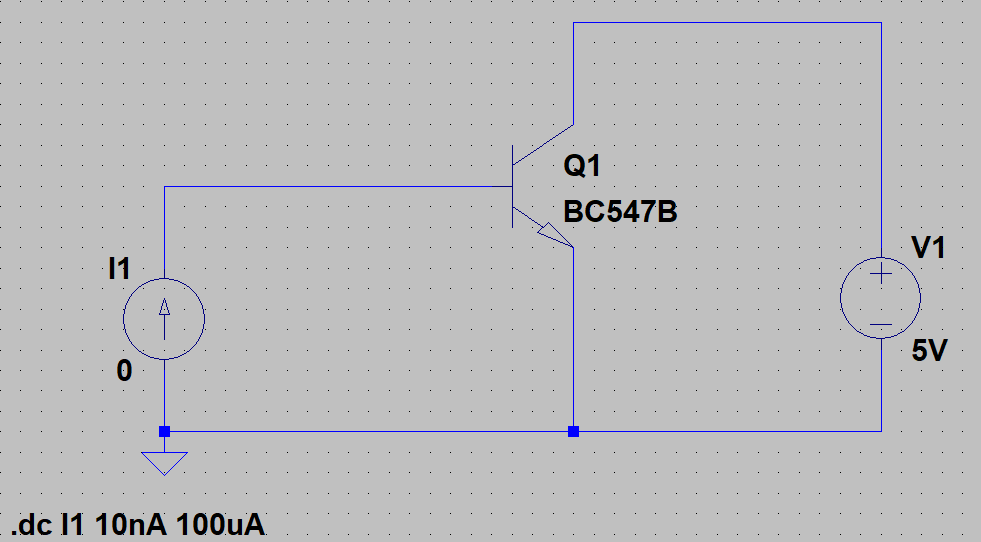
\includegraphics[width=0.5\linewidth]{Bilder/22aufbau.PNG}
            \caption{Schaltung zur Aufnahme des Eingangswiderstandes}
            \label{fig:22}
        \end{figure}

        Durch das Simulieren mit LT-Spice erhalten wir folgenden Graphen für den Eingangswiderstand. Die Werte sind doppellogarithmisch aufgetragen.

        \begin{figure}[!ht]
            \centering
            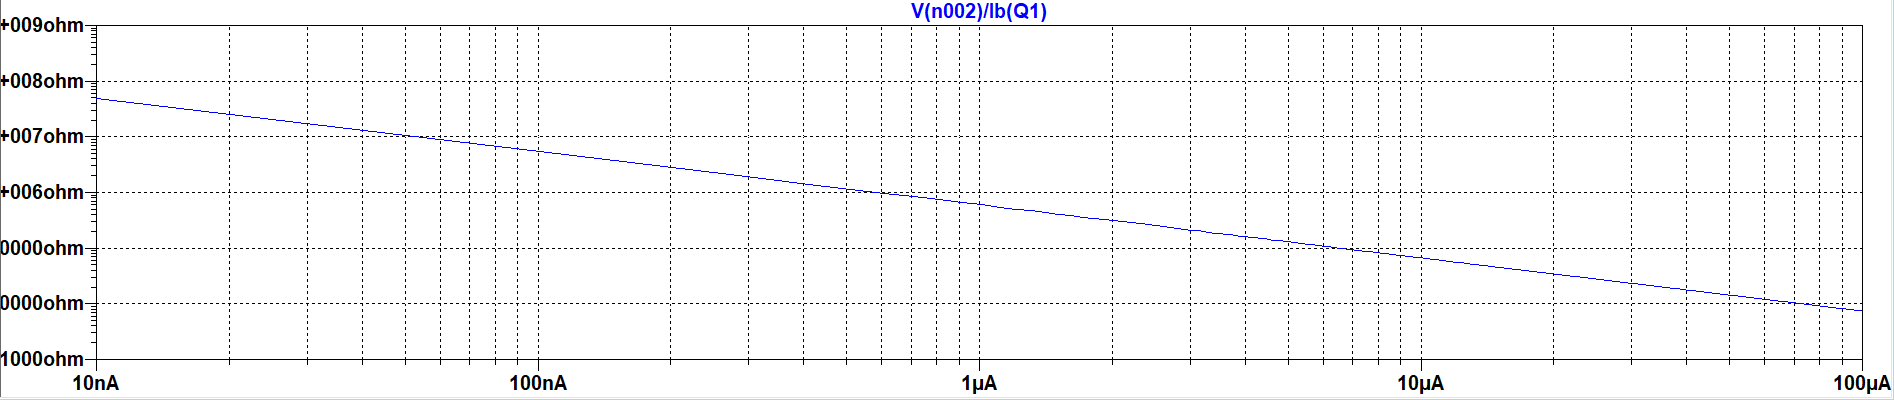
\includegraphics[width=\linewidth]{Bilder/22graph.PNG}
            \caption{Messwerte für \(r_{BE}=f(I_B)\)}
        \end{figure}

        Im Graphen ist zu erkennen, das der Eingangswiderstand mit steigender Stromstärke sinkt.

        \newpage
    \section{Aufnahme der Stromsteuerkennlinie}
        Um die Stromsteuerkennlinie \(I_C=f(I_B)\) zu ermitteln wird die selbe Schaltung verwendet \fref{fig:22}. Die Spannungsquelle V1 wird wieder mit 5 V versorgt. \(I_B\) wird dabei im Intervall von \(1\,\mu A\) bis \(1\,mA\) in der Simulation mit LT-Spice verändert. 

        \begin{figure}[!ht]
            \centering
            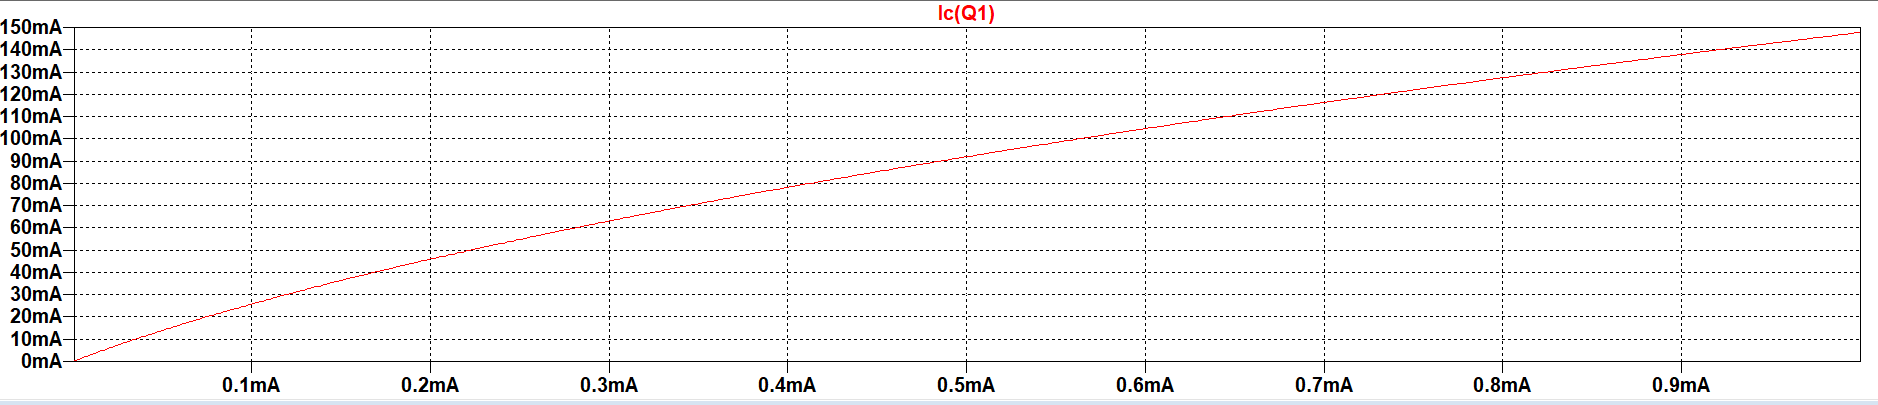
\includegraphics[width=\linewidth]{Bilder/23graph.PNG}
            \caption{Messwerte für den Kollektorstrom \(I_C\)}
        \end{figure}

        Im Graphen ist zu erkennen, dass der Kollektorstrom mit dem Basisstrom zusammen ansteigt. Dies geschieht jedoch nicht linear, sondern hat eine leichte Kurvenform.

    \section{Bestimmung der Stromverstärkung}
        Die Daten für \(I_B\) und \(I_C\) müssen mit LT-Spice aus dem Graphen entnommen werden.\\
        \url{https://raw.githubusercontent.com/wechlertj/hsrm_ap_bsc/master/WS2021/ET/Versuch_3/Stromstaerke.txt}\\
        Durch die Formel
        \begin{equation}
            \beta=\frac{I_C}{I_B}
        \end{equation}
        kann nun die Stromverstärkung ausgerechnet werden. Durch das Logarithmieren von \(I_C\) und \(\beta\) kann die Stromverstärkung als Funktion des Kollektorstroms in einem Diagramm dargestellt werden.

        \begin{figure}[!ht]
            \centering
            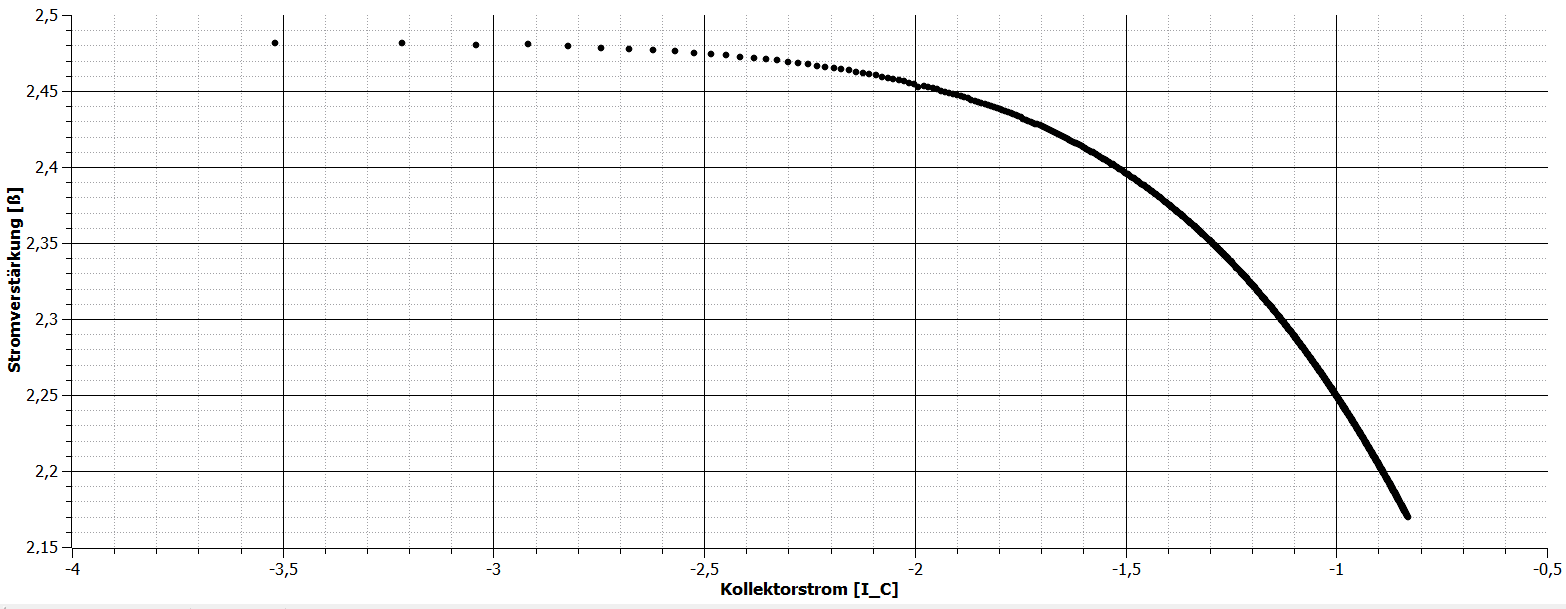
\includegraphics[width=\linewidth]{Bilder/24graph.PNG}
            \caption{Stromverstärkung als Funktion des Kollektorstroms doppellogarithmisch dargestellt}
            \label{fig:241}
        \end{figure}

        Im oben stehenden Link sind die einzelnen Messwerte und Ergebnisse für die Stromverstärkung und die einzelnen logarithmischen Funktionen zu sehen.

        \begin{figure}[!ht]
            \centering
            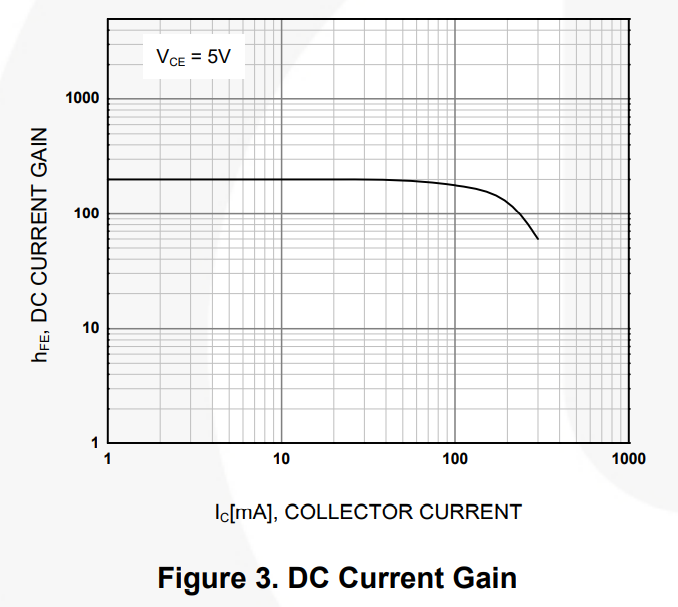
\includegraphics[]{Bilder/24datenblatt.PNG}
            \caption{Graph aus dem Datenblatt des Transistors BC547B \textbf{[B~\ref{fig:242}]}}
            \label{fig:242}
        \end{figure}

        Beim vergleichen der beiden Graphen~\ref{fig:241} und~\ref{fig:242} ist zu erkennen das diese fast gleich verlaufen. Beide laufen anfangs recht linear und ab einem bestimmtenKollektorstrom sinkt die Stromverstärkung rapide ab. Im Graph~\ref{fig:241} von beiden Achsen der Logarithmus genommen und dann aufgetragen, im Graph~\ref{fig:242} wurde das ganze im Graphen logarithmisch aufgezeichnet. Das Ergebnis ist das selbe.
        \newpage

    \section{Aufnahme der Ausgangskennlinienschar}
        Bei der Aufnahme der Kennlinienschar wird der gleiche Aufbau wie~\ref{fig:22} verwendet. Jedoch werden nun der Basisstrom I1 \(I_B\) und die Spannungsquelle V1 \(U_{CE}\) als veränderliche Größen verwendet. \(U_{CE}\) wird im Intervall von 0V bis 30V verändert und \(I_B\) im Intervall von 20 \(\mu A\) bis 100 \(\mu A\). Bei \(I_B\) wird schrittweise um 20 \(\mu A\) erhöht.

        \begin{figure}[!ht]
            \centering
            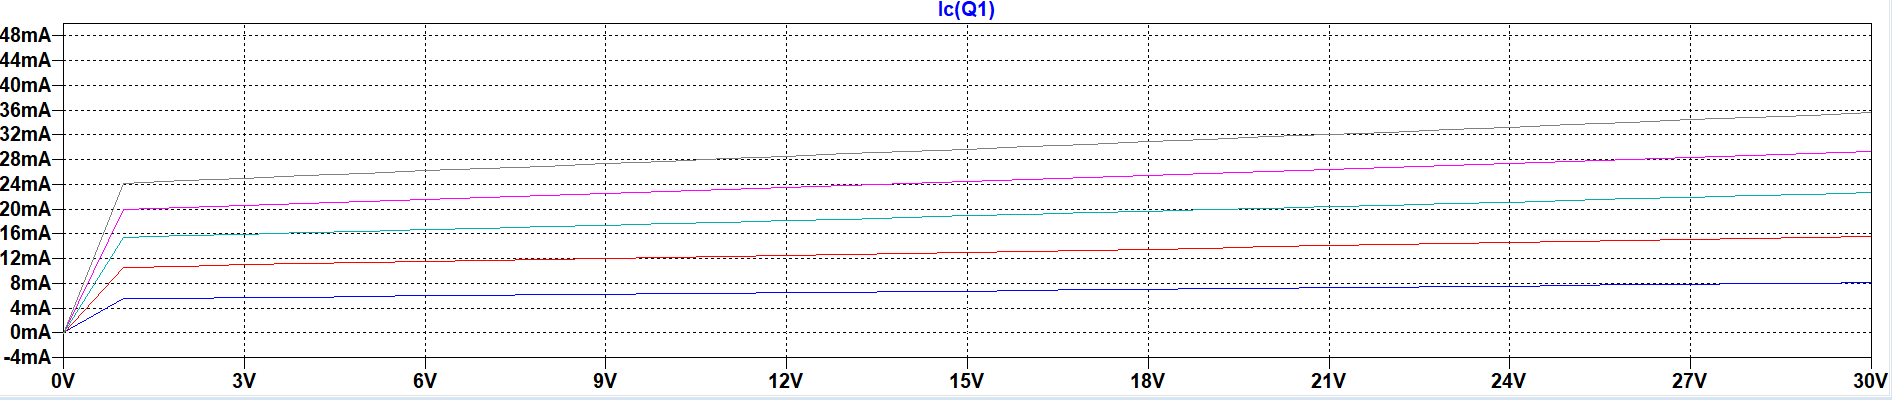
\includegraphics[width=\linewidth]{Bilder/25graph1.PNG}
            \caption{Ausgangskennlinien der verschiedenen Basisstromstärken}
            \label{fig:251}
        \end{figure}

        Aus dem Datenblatt des Transistors BC547B ist folgender Graph zu entnehmen.

        \begin{figure}[!ht]
            \centering
            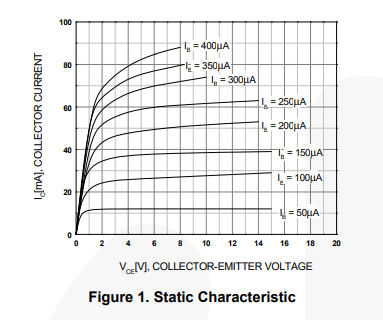
\includegraphics[]{Bilder/25datenblatt.PNG}
            \caption{Graph aus dem Datenblatt von BC547B \textbf{[B~\ref{fig:252}]}}
            \label{fig:252}
        \end{figure}

        Der von LT-Spice ermittelte Graph sieht nur ansatzweise so aus wie der Graph aus dem Datenblatt. Der ermittelte Kollektorstrom (Y-Achse) entspricht nicht den Werten aus dem Datenblatt. Jedoch sind die Intervalle für den Basisstrom im Intervall von \(50-100\,\mu A\) anders gewählt als in unserer Simulation. Deshalb kommen auch die anderen Werte für den Kollektorstrom zustande.\\
        Im folgenden Graph ist noch die Verlustleistungshyperbel für die Schaltung aufgezeigt.

        
        \begin{figure}[!ht]
            \centering
            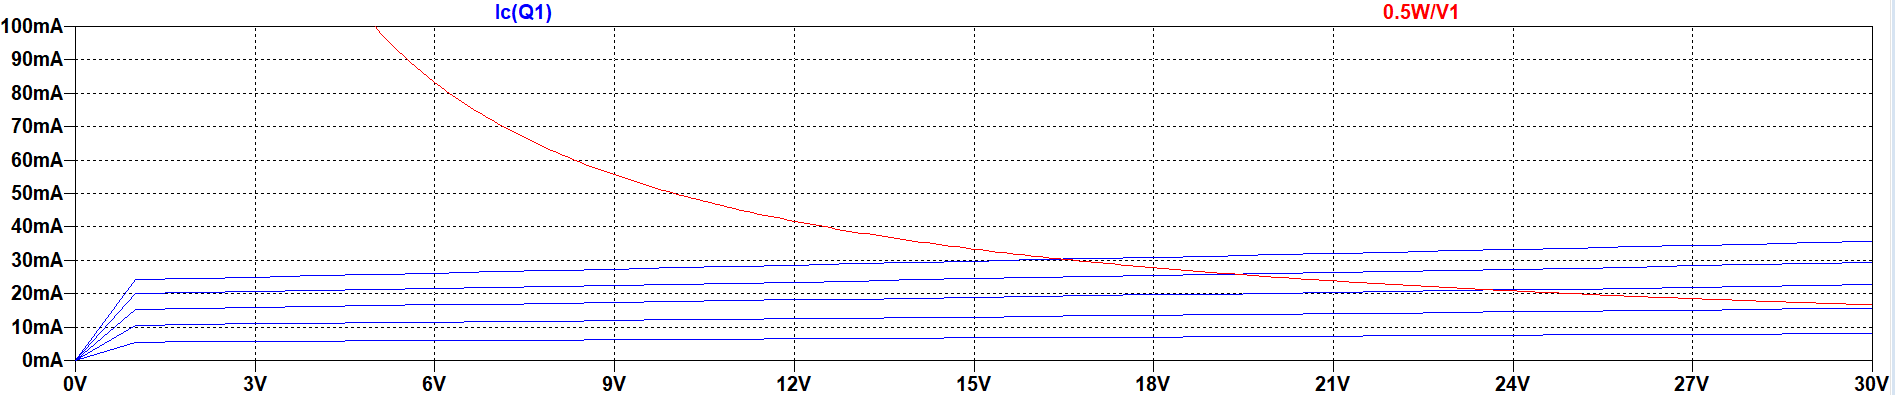
\includegraphics[width=\linewidth]{Bilder/25Verlustl.PNG}
            \caption{Verlustleistungshyperbel}
        \end{figure}

    \section{Bestimmung des differentiellen Ausgangswiderstands}
        Um den differentiellen Ausgangswiderstand \(r_{CE}\) wird die Simulation mit V1 (\(U_{CE}\)) im Intervall von 4V bis 6V und \(I_B\) im Intervall von 50 \(\mu A\) bis 350 \(\mu A\) in 50 \(\mu A\) durchgeführt. Für \(I_C\) kommen dabei folgende Werte heraus.\\
        \url{https://raw.githubusercontent.com/wechlertj/hsrm_ap_bsc/master/WS2021/ET/ Versuch_3/Ausgangswiderstand.txt}\\

        Durch die Formel 
        \begin{equation}
            r_{CE}=\frac{\Delta U_{CE}} {\Delta I_C}
        \end{equation}
        lässt sich der Ausgangswiderstand berechnen.

        Da der Strom immer von 4 V auf 6 V steigt ist \(\Delta U_{CE}= 2V\)

        Für die den Kollektorstrom \(\Delta I_C\) ergeben sich durch das Subtrahieren des Kollektorstroms bei U=4 V und U=6 V folgende Werte.
        \begin{equation}
            \Delta I_C=I_{Cmax}-I_{Cmin}
        \end{equation}

        \begin{table}[!ht]
        \centering
            \caption{Simulationsergebnisse \(\Delta I_C\)}
            \begin{tabular}{|c|c|}
                \hline
                \(I_B\) in \(\mu A\)& \(\Delta I_C\) in A\\ \hline \hline
                50 & 0.0004223 \\ \hline
                100 & 0.00078471\\ \hline
                150 & 0.00110695\\ \hline
                200 & 0.00139995\\ \hline
                250 & 0.00167042\\ \hline
                300 & 0.00192287\\ \hline
                350 & 0.00216047 \\ \hline
            \end{tabular}
        \end{table}

        Durch das Einsetzen der berechneten Werte in die Formel (1.2) ergibt sich für \(r_{CE}\):
        \begin{table}[!ht]
            \centering
            \caption{Simulationsergebnisse \(\Delta I_C\)}
            \begin{tabular}{|c|c|}
                \hline
                \(I_B\) in \(\mu A\)  & Wert von \(r_{CE}\) in \(\Omega\)\\
                \hline \hline
                50 & 4736 \\ \hline
                100 & 2549\\ \hline
                150 & 1807\\ \hline
                200 & 1429\\ \hline
                250 & 1197\\ \hline
                300 & 1040\\ \hline
                350 & 926\\ \hline
            \end{tabular}
        \end{table}
        \newpage
        Im Folgenden ist der Ausgangswiderstand \(r_{CE}\) in Abhängigkeit von dem Basisstrom \(I_B\) aufgetragen.

        \begin{figure}[!ht]
            \centering
            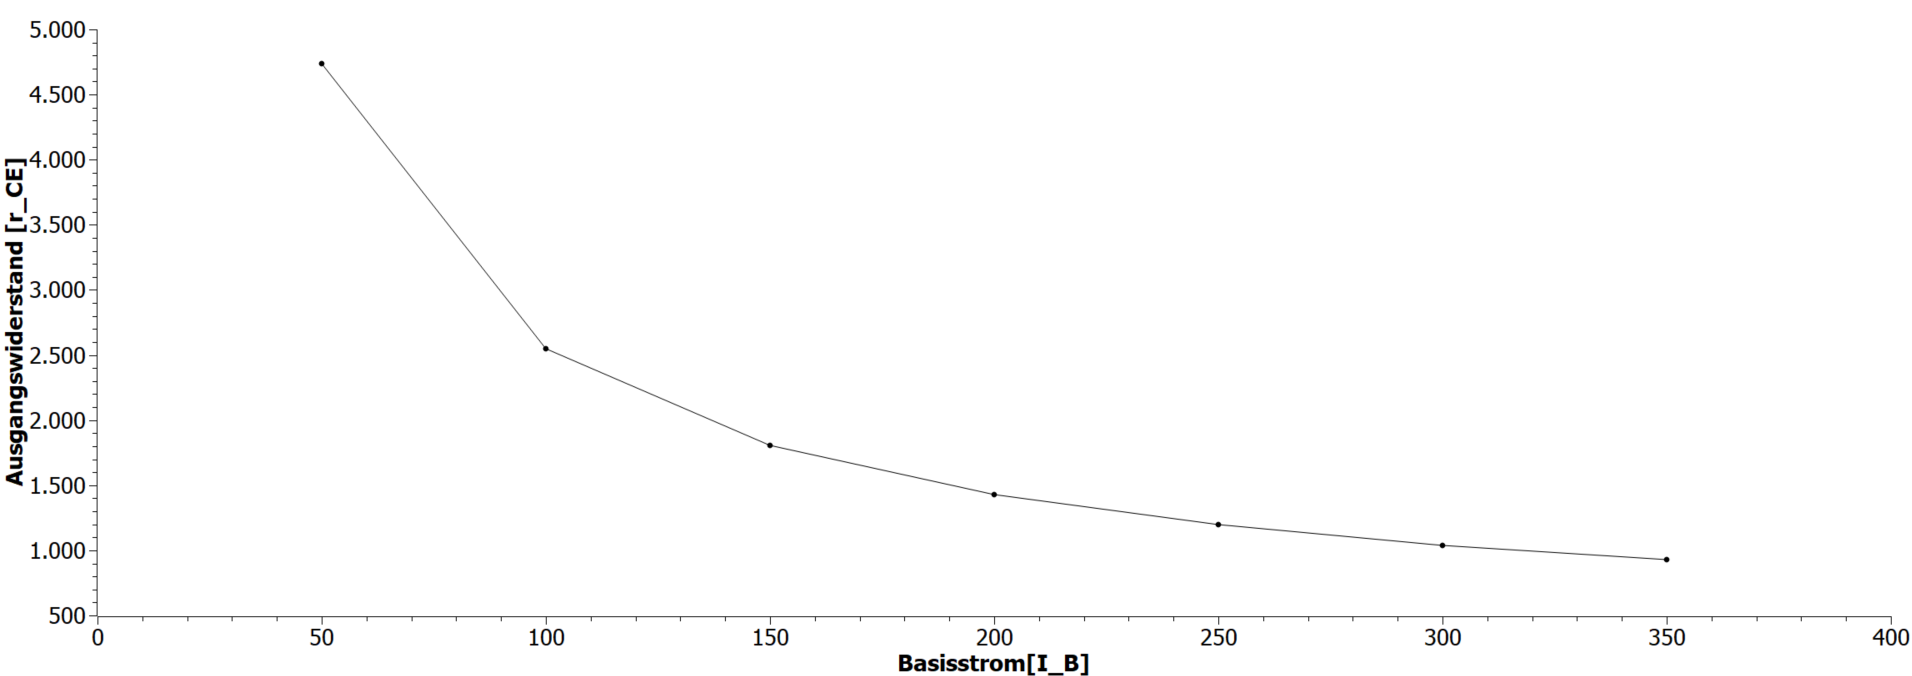
\includegraphics[width=\linewidth]{Bilder/26.PNG}
            \caption{Verhalten des Ausgangswiderstandes zum Basisstrom}
        \end{figure}









    \chapter{Fazit}
Bei dem Versuch werden erstmal die Grundlegenden Begriffe der Gleich- und Wechselspannung erklärt. 
Diese sind dann durch ein Voltmeter in die Schaltungen eingebracht worden. 
Dabei sind Schaltungen wie der Spannungsteiler und das Potentiometer aufgebaut worden 
und durch LTSpice simuliert. Zum besseren Verständnis des Graphen wurde 
dann der Effektivwert sowie die Ausgangsspannung per Hand ausgerechnet und mit den von 
LTSpice simulierten Werten verglichen. Die Werte für den Spannungsteiler und den Potentiometer
 haben mit den zu erwarteten Werten wunderbar funktioniert. Bei dem Rechtecksignal einer 
 Spannungsquelle sind jedoch zwischen simuliertem und berechneten Effektivwert Differenzen 
 aufgetreten. Ursprung des Fehlers kann in der Rechnung liegen, obwohl diese öfters zum Überprüfen 
 der Richtigkeit durchgeführt wurde. Der Fehler kann auch in der falschen Durchführung von 
 LTSpice liegen. In der Aufgabenstellung von 2.1 (Signalquellen), war nicht genau ersichtlich ob 
 das Voltmeter durch eine Wechselspannung oder Gleichspannung angetrieben wird. Durch eine 
 Wechselspannung würde der Graph von -1V bis 1V gehen. Die simulierten Graphen in dem Bericht 
 sind jedoch nur von 0V bis 1V aufgetragen. Durch die Wechselspannung sind die berechneten Werte 
 aber auch nicht zu erzielen, da diese ebenfalls zur Lösung des Problems simuliert wurden und 
 nicht mit den berechneten Werten übereinstimmen. 
    \chapter{Quellen}
\section*{Bilder}
\textbf{[B~\ref{fig:242}] und [B~\ref{fig:252}]}     https://www.onsemi.com/pub/Collateral/BC550-D.pdf\\
(18:03/10.01.2021)
   
    
    
    %\printbibliography
\end{document}